\documentclass[acmsmall]{acmart}
\usepackage{geometry}
\geometry{left=1in,right=0.75in,top=1in,bottom=1in}
\usepackage{graphicx}
\usepackage{datetime2}
\usepackage{amsmath}
\usepackage{titlesec}
\usepackage{tabularx}
\usepackage{hyperref}
\usepackage{indentfirst}
\usepackage{bm}
\usepackage{longtable}
\usepackage{xcolor}
\usepackage{colortbl}
\usepackage{etoolbox}
\definecolor{oddrow}{gray}{0.95}
\definecolor{evenrow}{gray}{0.98}
\titleformat*{\section}{\Large\bfseries\raggedright}
\title{Is P=NP:History and Frontier of NPC Problem}
\setcopyright{acmlicensed}
\copyrightyear{2025}
\acmYear{2025}
\acmDOI{1037103.7103710}
%1037,hhh
\acmJournal{JACM}
\acmVolume{1}
\acmNumber{1}
\acmArticle{1}
\acmMonth{1}
%Numbers here I set all 1~
\author{Xianzhe Meng}
\date{\today}
\email{U202410203@hust.edu.cn}
\orcid{0009-0009-9381-1315}
\affiliation{
	\institution{Huazhong University of Science and Technology}
	\city{Wuhan}
	\state{Hubei}
	\country{China}}
\newcounter{rowcount}
\setcounter{rowcount}{0}
\newcommand{\tablerow}[4]{%
	\stepcounter{rowcount}
	\ifodd\value{rowcount}
	\rowcolor{evenrow}
	\else
	\rowcolor{oddrow}
	\fi
	#1 & #2 & #3 & #4 \\
	\hline
}

\begin{document}

\renewcommand{\refname}{References}
\renewcommand{\tablename}{Table}

\renewenvironment{abstract}{
	\begin{center}
		\bfseries Abstract
		\vspace{0.5em}
	\end{center}
	\normalfont\small
}{%
	\par
}
	\graphicspath{{.}}
	\DeclareGraphicsExtensions{.pdf, .jpg, .tif, .png}
	\maketitle
	
	\begin{abstract}
		\setlength{\parskip}{-1em}
		This paper delves into the theoretical underpinnings and algorithmic strategies surrounding NP-complete (NPC) problems, with a particular emphasis on the \textit{P vs NP} conundrum. Emerging from Cook's 1971 demonstration of SAT's NP-completeness and Karp's subsequent reduction framework, NPC problems epitomize the most challenging problems within the NP class. The paper elucidates key complexity classes (P, NP, NPC, NP-hard), expounds NP-completeness through quintessential problems like TSP and Vertex Cover, and examines proof strategies for both \( P = NP \) (including algebraic methods) and \( P \neq NP \). It also contemplates practical solutions such as approximation algorithms and parameterized tractability, alongside real-world applications. Ultimately, the study accentuates the ongoing theoretical challenges and the interdisciplinary ramifications of NPC research.
		
	\end{abstract}
	\textbf{keywords}:NP-complete problems;time complexity;algorithm history
	
	\section{Introduction}
	In the course of computational science development, NP-complete problems have always occupied a pivotal position. Back in 1971, it was Stephen Cook who, in his groundbreaking paper \textit{The Complexity of Theorem Proving Procedures}\cite{cook1971complexity}, first introduced the concept of NP-completeness by proving SAT to be NP-complete. This achievement heralded an in-depth exploration of this unique class of problems. Subsequently, Richard Karp harnessed polynomial-time reductions to demonstrate that 21 classical combinatorial problems, such as TSP and VCP, also fall into the NP-complete category, thereby significantly broadening the scope of this theoretical domain. At the heart of NP-complete problems lies the contentious issue of \textit{"P vs NP"}. Designated as one of the \textit{Millennium Prize Problems} by the Clay Mathematics Institute with a reward of one million dollars for its solution\cite{claymillennium}, this question underscores the profound significance and elusiveness of NP-complete problems within the academic community.
	
	Over the past five decades, research on NP-complete problems has yielded fruitful results\cite{cormen2009introduction}. However, there still exists a paucity of systematic research that comprehensively reviews their historical development, key theoretical breakthroughs, and technological evolution.Our study endeavors to provide theoretical references and directional insights for future research. 
	\section{Definition and Origination}
	\subsection{SAT Problem}
	The Satisfiability Problem (SAT), a cornerstone in propositional logic, also stands as the first problem proven to be NP-complete in computational complexity theory. In propositional logic, formulas are constructed from variables (such as \(x_1, x_2, \ldots, x_n\)) and logical operators (\(\land\) for conjunction, \(\lor\) for disjunction, and \(\neg\) for negation).
	
	Given a propositional logic formula \(\varphi\), the SAT problem seeks to determine whether there exists an assignment of truth values (True/False) to the variables such that the formula \(\varphi\) evaluates to True. If such an assignment exists, the formula \(\varphi\) is deemed satisfiable; otherwise, it is unsatisfiable.
	
	In more rigorous mathematical terms, let \(X = \{x_1, x_2, \ldots, x_n\}\) denote the set of variables. A literal is either a variable \(x_i\) or its negation \(\neg x_i\). A clause is a disjunction (logical OR) of literals. For instance, \(C=(x_1\lor\neg x_2\lor x_3)\) represents a clause. A propositional formula \(\varphi\) is typically expressed in CNF, which is a conjunction of clauses:
	
	\begin{equation}
	\varphi = C_1\land C_2\land\cdots\land C_m=\bigwedge_{i = 1}^{m}C_i,\quad\text{where}\quad C_i=\bigvee_{j = 1}^{k_i}l_{ij}
	\end{equation}
	where \(l_{ij}\) signifies a literal, and \(k_i\) denotes the number of literals in clause \(C_i\). The objective of the SAT problem is to ascertain whether there exists a truth-value assignment \(\tau:X\rightarrow\{\text{True},\text{False}\}\) such that \(\tau(\varphi)=\text{True}\).
	
	In 1971, Stephen Cook established in his pioneering paper that the SAT problem is NP-complete \cite{cook1971complexity}. This conclusion was reached through the following two steps:
	\begin{enumerate}
		\item \textbf{SAT belongs to the class NP}: For any given truth-value assignment, we can verify whether this assignment satisfies the formula \(\varphi\) within polynomial time. It merely requires step-by-step computation of the truth value of \(\varphi\) in accordance with the rules of logical operators, with a time complexity of \(O(|\varphi|)\), where \(|\varphi|\) represents the length of the formula \(\varphi\).
		\item \textbf{Any problem in NP can be reduced to SAT}: Cook demonstrated that for any problem \(L\) in NP, there exists a polynomial-time reduction \(f\) such that \(x\in L\) if and only if \(f(x)\) is satisfiable. This implies that should a polynomial-time algorithm be discovered for solving the SAT problem, then all NP problems could be resolved in polynomial time.
	\end{enumerate}
	
	\subsection{What is NP Problem?}
	
	In the realm of complexity theory, decision problems revolve around being solved or verified within polynomial time. The definitions of these problems are based on their time complexity\cite{cormen2009introduction}.
	
	\textbf{P Problem}: Decision problems that can be solved in polynomial time.
	
	\textbf{NP Problem}: Decision problems for which a YES answer can be certified, and this certificate can be verified in polynomial time. However, it remains uncertain whether such problems can be solved in polynomial time.
	
	\textbf{NP-Complete(NPC) Problem}: An NP problem to which all other NP problems can be reduced. Solving an NPC problem would yield solutions for all NP problems.
	
	\textbf{NP-Hard Problem}: A problem \(H\) is NP-Hard if, for every \(L \in NP\), there exists a polynomial-time reduction from \(L\) to \(H\). Formally:
	\begin{equation}
	\forall L \in NP, \quad L \leq_p H
	\end{equation}
	where \(\leq_p\) represents a polynomial-time reduction.
	
	The relationships among these definitions are illustrated in Image1 and Image2:\\
	
	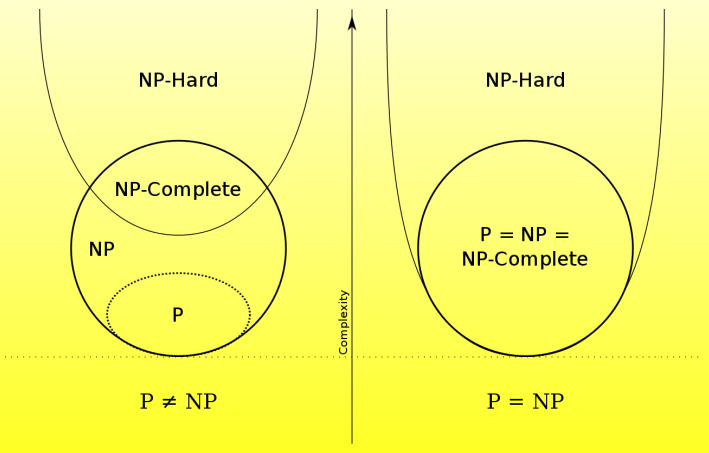
\includegraphics[width=0.5\textwidth]{1.png}
	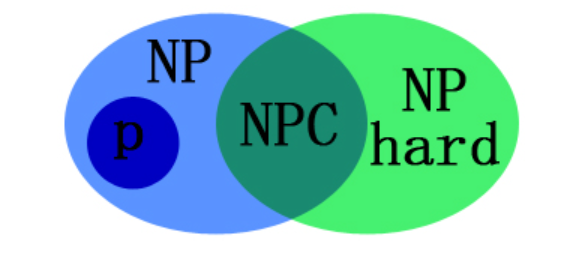
\includegraphics[width=0.5\textwidth]{2.png}
	\hspace*{9em} Image 1 \hspace*{17em} Image 2
	
	\subsection{History of Study}
	
	\begin{longtable}{|p{1.9cm}|p{1cm}|p{5.0cm}|p{4.0cm}|}
		
		\caption{Key Scientists and Study History of NP Problem\cite{cormen2009introduction}} \\
		\hline
		\rowcolor{oddrow}
		\textbf{Scientist} & \textbf{Year} & \textbf{Contribution} & \textbf{Significance} \\
		\hline
		\endfirsthead
		
		\multicolumn{4}{r}{\textit{Continued from previous page}} \\
		\hline
		\rowcolor{oddrow}
		\textbf{Scientist} & \textbf{Year} & \textbf{Contribution} & \textbf{Significance} \\
		\hline
		\endhead
		
		\hline
		\multicolumn{4}{r}{\textit{Continued on next page}} \\
		\endfoot
		
		\hline
		\endlastfoot
		\rowcolor{evenrow}
		Manuel Blum & 1967 & Developed Blum complexity theory. & Established the foundational tools. \\
		\hline
		\rowcolor{oddrow}
		Stephen Cook & 1971 & Demonstrated the NP-completeness of SAT in "The Complexity of Theorem-Proving Procedures". & Established the concept of NPC. \\
		\hline
		\rowcolor{evenrow}
		Richard Karp & 1972 & Linked 21 problems to NP-completeness through reductions. & Expanded the scope of NP-hardness. \\
		\hline
		\rowcolor{evenrow}
		Leonid Levin & 1973 & Independently discovered NP-completeness. & Reinforced the theoretical foundation. \\
		\hline
		\rowcolor{oddrow}
		Mihir Bellare & 1993 & Contributed to the PCP theorem. & Connected NP to proof complexity. \\
		\hline
		\rowcolor{evenrow}
		Christos Papadimitriou & 1994 & Co-authored \textit{Computational Complexity}. & Formalized complexity theory. \\
		\hline
		\rowcolor{oddrow}
		Johan Håstad & 1997 & Proved inapproximability results for MAX-3SAT. & Set limits on approximation algorithms. \\
		\hline
		\rowcolor{evenrow}
		Oded Goldreich & 2001 & Linked NP to cryptography in \textit{Foundations of Cryptography}. & Enabled practical applications. \\
		\hline
		\rowcolor{oddrow}
		Dana Moshkovitz & 2019 & Advanced derandomization techniques. & Bridged the gap between P and NP. \\
		\hline
	\end{longtable}
	
	\section{Classical Examples}
	\subsection{TSP}
	
	The Traveling Salesman Problem (TSP) stands as a classic combinatorial optimization problem. Given a set of \(n\) cities and the distances \(d(i, j)\) between each pair of cities \(i\) and \(j\), the objective is to identify the shortest possible route that visits each city exactly once and returns to the origin city. Mathematically, representing the route as a permutation \(\pi = (\pi_1, \pi_2, \ldots, \pi_n)\) of the cities, where \(\pi_1\) denotes the starting city and \(\pi_{n + 1}=\pi_1\), the goal is to minimize the total distance:
	\[
	\text{Minimize} \quad \sum_{i = 1}^{n} d(\pi_i, \pi_{i + 1})
	\]
	
	The TSP manifests in two primary variants:
	\begin{enumerate}
		\item \textbf{Symmetric TSP}: \(d(i, j)=d(j, i)\) for all \(i\) and \(j\), implying that the distance from city \(i\) to city \(j\) is identical to that from \(j\) to \(i\).
		\item \textbf{Asymmetric TSP}: \(d(i, j)\neq d(j, i)\) in general, often emerging in transportation networks with one-way streets or varying travel times in opposite directions.
	\end{enumerate}
	
	\subsubsection{Early Conceptions and Origins (1800s - 1930s)}
	
	\hspace{1.2em}The concept of the TSP can be traced back to the 19th century.\cite{J2014The} In 1832, a German textbook on traveling salesmanship outlined a problem akin to the TSP, albeit not formalized as a mathematical problem. The first formal study of the TSP is attributed to the Irish mathematician William Rowan Hamilton and the British mathematician Thomas Kirkman in the 1850s. Hamilton's Icosian game, which involved finding a cycle that traverses each vertex of a dodecahedron exactly once, served as a precursor to the TSP. However, it focused on the existence of a cycle rather than optimizing a cost function.
	
	The modern formulation of the TSP as an optimization problem emerged in the 1930s, primarily within the context of operations research and industrial applications. Mathematicians and researchers began to explore how to efficiently plan routes for salesmen, delivery trucks, and other scenarios requiring traversal of multiple locations in an optimal manner.
	
	\subsubsection{Exact Algorithms: Early Approaches (1950s - 1960s)}
	
	\hspace{1.2em}In the early stages of research, exact algorithms for the TSP centered on brute-force search and dynamic programming.
	\begin{itemize}
		\item \textbf{Brute - Force Search}: The most straightforward approach involves enumerating all possible permutations of the \(n\) cities and calculating the total distance of each tour. However, this method entails a time complexity of \(\Theta(n!)\), rendering it impractical even for moderately large \(n\). For example, when \(n = 20\), there are \(20!\approx 2.43\times 10^{18}\) potential tours\cite{J2014The}.
		
		\item \textbf{Held - Karp Algorithm (1962)}: Developed by Michael Held and Richard M. Karp, this dynamic programming algorithm addresses the TSP with a time complexity of \(\Theta(n^2 2^n)\)\cite{held1962dynamic}. It operates by computing the shortest path to each subset of cities, effectively reducing the search space compared to brute-force methods. Despite its exponential nature, it marked a significant improvement for small-to-medium-sized instances and remains a benchmark for exact TSP solvers.
	\end{itemize}
	
	\subsubsection{Computational Complexity and NP - Completeness (1970s)}
	
	\hspace{1.2em}In 1972, Richard Karp established the NP - Hardness of the TSP in his seminal paper "Reducibility Among Combinatorial Problems"\cite{karp1972reducibility}. He demonstrated that the decision version of the TSP (i.e., given a distance bound \(k\), does there exist a tour with a total distance of at most \(k\)) is NP - Complete. This implies that should a polynomial - time algorithm be found for the TSP, it would entail \(P = NP\), thereby resolving one of the most significant open problems in computer science. This proof represented a major milestone, as it positioned the TSP as a fundamental problem in computational complexity studies.
	
	\subsubsection{Heuristic and Approximation Algorithms (1970s - Present)}
	
	\hspace{1.2em}Given the computational expense of exact algorithms for large \(n\), researchers have developed numerous heuristic and approximation algorithms to obtain near - optimal solutions within polynomial time \cite{yilmaz2020analysis}.
	\begin{itemize}
		\item \textbf{Christofides' Algorithm (1976)}: One of the most renowned approximation algorithms for the metric TSP (where distances satisfy the triangle inequality, \(d(i, j)+d(j, k)\geq d(i, k)\) for all \(i\), \(j\), \(k\)), Christofides' algorithm ensures a solution no more than \(1.5\) times the optimal tour length\cite{christofides1976worst}. It integrates minimum spanning trees, matching, and path - merging techniques.
		
		\item \textbf{2 - Opt Heuristic (1950s)}: A simple yet effective local search heuristic. Starting with an initial tour, it iteratively enhances the tour by removing two edges and reconnecting the remaining paths in an alternative manner to reduce the total distance. Although it does not guarantee optimality, it can swiftly identify good solutions and is frequently employed as a subroutine in more complex algorithms.
		
		\item \textbf{Metaheuristics}: In recent decades, metaheuristics such as genetic algorithms, simulated annealing, and ant colony optimization have been extensively applied to the TSP. Drawing inspiration from natural phenomena (e.g., evolution, annealing in physics, ant foraging behavior), these algorithms more effectively explore the solution space. For instance, genetic algorithms utilize operations like crossover and mutation on a population of candidate tours to evolve better solutions over time.
	\end{itemize}
	
	\subsubsection{Modern Developments and Applications}
	
	\hspace{1.2em}With the advancement of computing power and the emergence of new technologies, TSP research continues to evolve:
	\begin{itemize}
		\item \textbf{Parallel and Distributed Computing}: Researchers have investigated parallelizing TSP algorithms to leverage multi - core processors and distributed computing systems. This enables faster computation of solutions, particularly for large - scale instances.
		
		\item \textbf{Machine Learning and Data - Driven Approaches}: Recent research has explored employing machine learning techniques to predict good solutions for the TSP. For example, neural networks can be trained on a set of TSP instances to identify patterns and generate near - optimal tours more efficiently.
	\end{itemize}
	
	In conclusion, the Traveling Salesman Problem has served as a central topic in combinatorial optimization and computational complexity for over a century. Despite significant progress in algorithm development and complexity understanding, the pursuit of more efficient solutions and the quest to prove or disprove \(P = NP\) continue to drive research in this field.
	
	\subsection{VCP}
	
	The Vertex Cover Problem (VCP) constitutes a fundamental combinatorial optimization problem in graph theory\cite{2020Parameterized}. Given an undirected graph \( G = (V, E) \) with vertex set \( V \) and edge set \( E \), a vertex cover is a subset \( C \subseteq V \) such that every edge \( e \in E \) is incident to at least one vertex in \( C \). The objective is to identify the smallest possible vertex cover (minimum vertex cover). Formally:
	
	\textbf{Vertex Cover}:
	A subset \( C \subseteq V \) qualifies as a vertex cover if for every edge \( (u, v) \in E \), either \( u \in C \) or \( v \in C \) (or both). The minimum vertex cover problem seeks to minimize \( |C| \).
	
	The decision version of VCP inquires:
	\begin{quote}
		Given a graph \( G \) and an integer \( k \), does there exist a vertex cover \( C \) with \( |C| \leq k \)?
	\end{quote}
	
	\subsubsection{Early Conceptions and Origins (1970s)}
	
	\hspace{1.2em}The formal investigation of the Vertex Cover Problem emerged in the 1970s as part of the broader exploration into NP-completeness. The problem was among the first 21 problems proven to be NP-complete by Richard Karp in his landmark 1972 paper\cite{karp1972reducibility} . Although the concept of vertex covers dates back to earlier graph theory research, its classification as a canonical NP-complete problem solidified its importance in computational complexity theory.
	
	\subsubsection{Exact Algorithms: Early Approaches (1970s-1990s)}
	\hspace{1.2em}Initial efforts to solve VCP centered on exact algorithms, primarily through brute-force enumeration and dynamic programming:
	\begin{itemize}
		\item \textbf{BFS}: This simplest approach involves checking all subsets of vertices of size \( k \) for \( k \) ranging from 1 to \( |V| \). However, it entails a time complexity of \( \Theta(2^n \cdot m) \), where \( n = |V| \) and \( m = |E| \), rendering it infeasible for large graphs.
		
		\item \textbf{Buss's Kernelization (1993)}: An early parameterized algorithm by Buss\cite{Josep2006Kernels} demonstrated that VCP can be reduced to an equivalent instance (kernel) of size \( \Theta(k^2) \) in polynomial time, leading to an \( \Theta(2^k \cdot k^2 + n^2) \) algorithm for fixed \( k \). This represented a significant improvement for small \( k \).
	\end{itemize}
	
	\subsubsection{Computational Complexity and NP-Completeness (1970s)}
	\hspace{1.2em}Karp's 1972 reduction from 3-SAT to VCP established its NP-completeness. This proof demonstrated that any instance of 3-SAT (a known NP-complete problem) can be transformed into an equivalent instance of VCP in polynomial time\cite{karp1972reducibility} . This result had profound implications for approximation algorithms, as it suggested that VCP is unlikely to possess a polynomial-time exact solution unless \( P = NP \).
	
	\subsubsection{Approximation Algorithms (1970s-Present)}
	\hspace{1.2em}Owing to its NP-hardness, research shifted towards polynomial-time approximation algorithms:
	
	\begin{itemize}
		\item \textbf{2-Approximation (1970s)}: A simple greedy algorithm that repeatedly selects an edge and adds both its endpoints to the cover yields a 2-approximation\cite{garey1979computers}. This remains one of the most widely utilized algorithms for practical applications.
		
		\item \textbf{LP-Based Approximation (1980s)}: Utilizing linear programming relaxation, researchers developed a \( \frac{2}{3} \)-approximation algorithm for bipartite graphs.\cite{1998An}
		
		\item \textbf{Inapproximability Results (2005)}: Dinur and Safra demonstrated that VCP cannot be approximated within a factor of \( 1.36 \) unless \( P = NP \)\cite{dinur2005analytical}. This result established a theoretical limit on approximation algorithms.
	\end{itemize}
	
	\subsubsection{Parameterized Complexity (1990s-Present)}
	\hspace{1.2em}The emergence of parameterized complexity theory led to significant advancements for VCP:
	
	\begin{itemize}
		\item \textbf{Fixed-Parameter Tractable (FPT) Algorithms}: In 1995, Chen et al. developed an \( \Theta(1.286^k \cdot n) \) algorithm employing branching and kernelization techniques\cite{chen2006improved}. Subsequent improvements reduced the exponent to \( \Theta(1.2738^k + kn) \) \cite{fomin2016exact}.
		
		\item \textbf{Kernelization Lower Bounds}: In 2014, Dell and van Melkebeek established that VCP does not admit a polynomial kernel unless \( NP \subseteq coNP/poly \)\cite{2014Satisfiability}.
	\end{itemize}
	
	\subsubsection{Modern Developments and Applications}
	
	\hspace{1.2em}Recent research has concentrated on algorithmic engineering, parallel and distributed algorithms, machine learning, and heuristics. These advancements have deepened our understanding of VCP and facilitated numerous real-world applications, including:
	\begin{enumerate}
		\item Sensor networks (minimizing active nodes while covering all edges).
		\item Fault detection in circuits (identifying critical components).
		\item Social network analysis (identifying influencers in viral marketing).
	\end{enumerate}
	
	In summary, the Vertex Cover Problem has served as a cornerstone of computational complexity theory for decades. Its study has driven innovations in approximation algorithms, parameterized complexity, and practical optimization techniques. While exact solutions remain intractable for large graphs, ongoing research continues to expand the boundaries of computational feasibility.
	
	\section{Algorithmic Strategies}
	\subsection{Proof Strategies for \( P = NP \)}
	
	Establishing \( P = NP \) necessitates either constructing a polynomial-time algorithm for an NP-complete problem \( \Pi \in \text{NPC} \) or demonstrating that non-deterministic Turing machines (NTMs) can be simulated deterministically within polynomial time. Below are the principal approaches:
	
	\subsubsection{Constructive Algorithms for NP-Complete Problems}
	\paragraph{}\hspace{0.8em}The most straightforward method involves designing a polynomial-time algorithm for an NP-complete problem, such as 3-SAT or TSP.
	
	\paragraph{\textbf{Algebraic Methods}}
	\hspace{0.7em}Translating NP-complete problems into algebraic systems represents one approach. For example, encoding a 3-SAT formula \( \phi \) as a system of polynomial equations over the finite field \(F_2\):
	\begin{equation}
		\phi(x_1,\ldots,x_n) \equiv \bigwedge_{i=1}^m  C_i(x_1,\ldots,x_n)
	\end{equation}
	Each clause \( C_i \) corresponds to a polynomial constraint. Should such systems be solvable in \( \Theta(p(n)) \) time for some polynomial \( p \), it would imply \( P = NP \). However, general polynomial system solving is NP-hard, and no efficient algorithm is currently known.
	
	\paragraph{\textbf{Quantum Computing}}
	
	\hspace{0.7em}Quantum algorithms leverage superposition and entanglement to explore solution spaces. For instance, Shor's algorithm factors integers in \( \Theta((\log N)^3) \) time, exponentially faster than classical algorithms. Nevertheless, no quantum algorithm has yet solved an NP-complete problem in polynomial time. Quantum annealing shows promise for optimization but lacks theoretical guarantees for \( P = NP \).
	
	\paragraph{\textbf{Structural Insights}}
	
	\hspace{0.7em}Exploiting hidden structures within NP-complete problems presents another avenue. For example, planar graphs admit polynomial-time solutions for certain NP-complete problems, such as 4-colorability (decidable in \( \Theta(n^2) \) time ) and TSP (approximable within a factor of \( 1 + \varepsilon \) in polynomial time ). However, these results do not generalize to arbitrary graphs.
	
	\subsubsection{Logical and Meta-Complexity Approaches}
	
	\paragraph{\textbf{Simulating Non-Determinism}}
	
	\hspace{0.7em}Proving that the exponential branching of NTMs can be compressed into polynomial time stands as a key direction. Approaches include derandomization, where the hypothesis \( \text{NP} \subseteq \text{BPP} \) combined with robust pseudorandom generator (PRG) assumptions (e.g., \( \text{E} \) requiring circuits of size \( 2^{\Omega(n)} \)) would imply \( \text{NP} \subseteq \text{P} \). Alternatively, combinatorial bounds on the number of accepting paths in an NTM, utilizing techniques like expander graphs, could facilitate polynomial-time simulations.
	
	\paragraph{\textbf{Logical Characterizations}}
	
	\hspace{0.7em}Relating \( P \) and \( NP \) to logical systems offers another perspective. For example, Fagin's Theorem posits that \( NP \) comprises the set of languages expressible in existential second-order logic. A proof demonstrating that \( P \) and \( NP \) coincide within a logical framework (e.g., fixed-point logic with counting) would resolve the \( P \text{ vs } NP \) problem.
	
	\subsection{Proof Strategies for \( P \neq NP \)}
	
	Demonstrating \( P \neq NP \) requires showing that some \( \Pi \in NP \) demands super-polynomial time. Key approaches encompass:
	
	\paragraph{\textbf{Diagonalization and Oracle Separations}}
	
	\hspace{0.7em}Classical diagonalization, which constructs a language \( L \in NP \) that diagonalizes against all polynomial-time DTMs, fails due to the relativization barrier: oracles \( A \) and \( B \) exist such that \( P^A = NP^A \) and \( P^B \neq NP^B \). This indicates that any proof of \( P \neq NP \) must employ non-relativizing techniques. While interactive proof systems, such as \( \text{MIP*} = \text{RE} \), provide insights into complexity class separations, they are too powerful to directly imply \( P \neq NP \).
	
	\paragraph{\textbf{Circuit Complexity}}
	
	\hspace{0.7em}Establishing super-polynomial lower bounds on the size of Boolean circuits required to compute NP-complete functions represents a central approach. Razborov's 1985 result showed that monotone circuits for CLIQUE require size \( 2^{\Omega(n^{1/4})} \), but this does not extend to general circuits. The natural proofs barrier posits that any "natural" proof of a circuit lower bound would violate cryptographic assumptions. Similarly, the algebrization barrier\cite{Scott2009Algebrization}demonstrates that techniques employing linear algebra or arithmetization cannot separate \( P \) and \( NP \).
	
	\paragraph{\textbf{Proof Complexity}}
	
	\hspace{0.7em}Associating the difficulty of solving NP problems with the length of their proofs in formal systems presents another avenue. For example, proving that tautologies encoding NP-hard problems (e.g., TSP) require super-polynomial-length proofs in extended Frege systems would imply \( NP \neq coNP \), a result stronger than \( P \neq NP \). Craig's interpolation theorem links proof complexity and circuit complexity, yet no such lower bounds are known for NP-complete problems.
	
	\section{Conclusion and Further Thinking}
	
	Since the formalization of NP-completeness over four decades ago, these problems have remained central to theoretical computer science. Foundational work by Cook in 1971 and Karp in 1972 revealed that a wide array of combinatorial decision problems (e.g., SAT, TSP, Vertex Cover) are all inter-reducible, forming the class of the "hardest problems in NP" \cite{karp1972reducibility}. As Garey and Johnson emphasized, the question of whether these NP-complete problems are inherently intractable stands as "one of the foremost open questions of contemporary mathematics and computer science" \cite{garey1979computers}. Thus, the P versus NP problem has become a touchstone for understanding the limits of efficient computation.
	
	Over the years, a vast body of research has developed around NP-complete problems.Despite this extensive research, the fundamental P vs NP question remains unresolved. But we have research on how NPC problem can be solved,which is summarized in this paper.
	
	Beyond theory, NP-complete problems have profound practical relevance. Classic examples like the Boolean satisfiability problem, the traveling salesman problem, and the Vertex Cover problem emerge in diverse applications. For instance, the Steiner tree problem (an NP-hard variant closely related to vertex cover) has direct applications in circuit design and network topology\cite{sipser2012introduction}. Therefore,research on NP-complete problems remains a fertile frontier.Study on NPC problem should be emphasized,which remains important to human society.
	
\bibliographystyle{ACM-Reference-Format}
\bibliography{reference}

\end{document}